% This file was created by tikzplotlib v0.9.8.
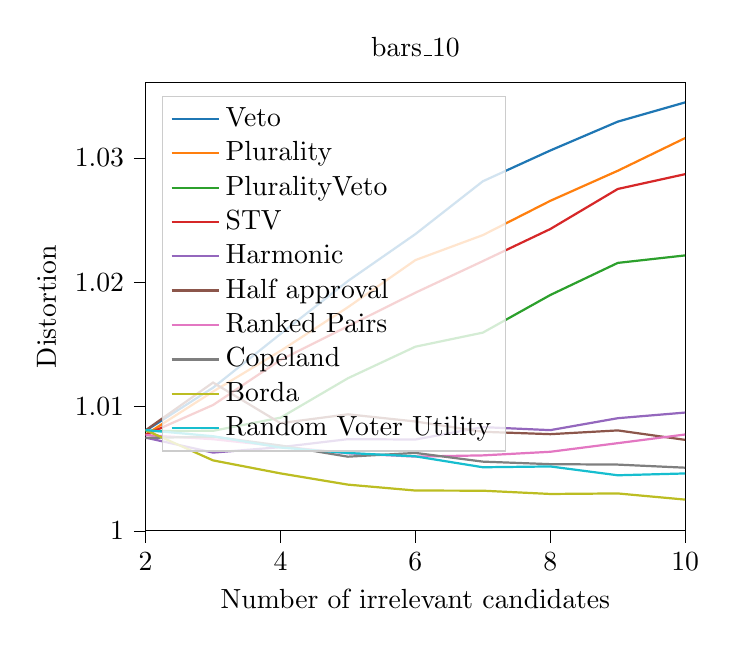
\begin{tikzpicture}

\definecolor{color0}{rgb}{0.12156862745098,0.466666666666667,0.705882352941177}
\definecolor{color1}{rgb}{1,0.498039215686275,0.0549019607843137}
\definecolor{color2}{rgb}{0.172549019607843,0.627450980392157,0.172549019607843}
\definecolor{color3}{rgb}{0.83921568627451,0.152941176470588,0.156862745098039}
\definecolor{color4}{rgb}{0.580392156862745,0.403921568627451,0.741176470588235}
\definecolor{color5}{rgb}{0.549019607843137,0.337254901960784,0.294117647058824}
\definecolor{color6}{rgb}{0.890196078431372,0.466666666666667,0.76078431372549}
\definecolor{color7}{rgb}{0.737254901960784,0.741176470588235,0.133333333333333}
\definecolor{color8}{rgb}{0.0901960784313725,0.745098039215686,0.811764705882353}

\begin{axis}[
legend cell align={left},
legend style={
  fill opacity=0.8,
  draw opacity=1,
  text opacity=1,
  at={(0.03,0.97)},
  anchor=north west,
  draw=white!80!black
},
tick align=outside,
tick pos=left,
title={bars\_10},
x grid style={white!69.0196078431373!black},
xlabel={Number of irrelevant candidates},
xmin=2, xmax=10,
xtick style={color=black},
y grid style={white!69.0196078431373!black},
ylabel={Distortion},
ymin=1, ymax=1.03606019149108,
ytick style={color=black}
]
\addplot [thick, color0]
table {%
2 1.00804920301524
3 1.01151180274057
4 1.01583544368037
5 1.02009421913783
6 1.02386636912267
7 1.02811552715437
8 1.03059161538283
9 1.03291114783494
10 1.03446254742509
};
\addlegendentry{Veto}
\addplot [thick, color1]
table {%
2 1.00773355208709
3 1.01120072282267
4 1.0144704640676
5 1.0179864564286
6 1.02177470785398
7 1.02378498439077
8 1.0265429535587
9 1.02896013224621
10 1.03159312602639
};
\addlegendentry{Plurality}
\addplot [thick, color2]
table {%
2 1.00802688362228
3 1.00804292550128
4 1.00909957317079
5 1.01227290622213
6 1.01481055457778
7 1.01594156247384
8 1.01896710652472
9 1.02154886295886
10 1.02215199706422
};
\addlegendentry{PluralityVeto}
\addplot [thick, color3]
table {%
2 1.00772538883024
3 1.01011994201097
4 1.01374586979144
5 1.01645724527763
6 1.01915259225157
7 1.02169265915167
8 1.02427442643403
9 1.02749515040497
10 1.02868897974894
};
\addlegendentry{STV}
\addplot [thick, color4]
table {%
2 1.00749686687038
3 1.00629250732687
4 1.00672776320145
5 1.00737282372507
6 1.00734388864891
7 1.00834174164106
8 1.00809757416768
9 1.00905837385098
10 1.00951216403556
};
\addlegendentry{Harmonic}
\addplot [thick, color5]
table {%
2 1.00808523860217
3 1.01192556625684
4 1.00865945483639
5 1.00937049468322
6 1.00879382425946
7 1.00796447026343
8 1.00777390190343
9 1.00807580198758
10 1.00731473926972
};
\addlegendentry{Half approval}
\addplot [thick, color6]
table {%
2 1.00770413961558
3 1.00736728436162
4 1.00679097493193
5 1.00623157352451
6 1.00597193133167
7 1.00606710315275
8 1.00635717219229
9 1.00705083182945
10 1.00774832484292
};
\addlegendentry{Ranked Pairs}
\addplot [thick, white!49.8039215686275!black]
table {%
2 1.00747262830742
3 1.0075724174523
4 1.00686289202759
5 1.00596395915943
6 1.00626533763651
7 1.00556487536871
8 1.00536134353116
9 1.00532579243307
10 1.00507701467833
};
\addlegendentry{Copeland}
\addplot [thick, color7]
table {%
2 1.00810007960707
3 1.00566456328519
4 1.00461836683392
5 1.00371473040028
6 1.00323946269427
7 1.00322700767377
8 1.00296354492565
9 1.00300558128704
10 1.00250966610525
};
\addlegendentry{Borda}
\addplot [thick, color8]
table {%
2 1.00810574855809
3 1.00760892451477
4 1.00669701193981
5 1.00625992785476
6 1.00598963384795
7 1.00511236023402
8 1.00517679888989
9 1.00446749355356
10 1.00461423534397
};
\addlegendentry{Random Voter Utility}
\end{axis}

\end{tikzpicture}
